% Block 5 of lista-reais-lectures-01-05 (input by the drivers in Listas/).
% Order and ratings: lista-reais-lectures-01-05/order.md.
\bloco{5}{Repeated games and bargaining}{Lecture 5}

% ---------------------------------------------------------------------------
\exercicio[1]{Finitely repeated game}{Foundations}{Cabral (2017), \emph{Introduction to Industrial
Organization}, 2nd ed., Ch.~7 ``Games and Strategies'', Exercises, Exercise 7.13 ``Finitely repeated
game'', p.~182 [PDF 194]. No answer in the book. Reproduced verbatim.}

\rot{7.13.}\textbf{Finitely repeated game.} Suppose that the game depicted in Figure 7.1 is repeated
$T$ times, where $T$ is known. Show that the only subgame perfect equilibrium is for players to
choose $(B, R)$ in every period.

\begin{referencia}{``the game depicted in Figure 7.1'': Cabral (2017), Ch.~7, Figure 7.1 ``The
`prisoner's dilemma' game'' and the sentence that explains how its cells are read, p.~160 [PDF 172].
Figure cropped from the page; text reproduced verbatim.}
For each combination of strategies by each player, the respective matrix cell shows the payoffs
received by each player. In the lower left corner, the payoff received by Player 1; in the top right
corner, the payoff received by Player 2.
\begin{center}
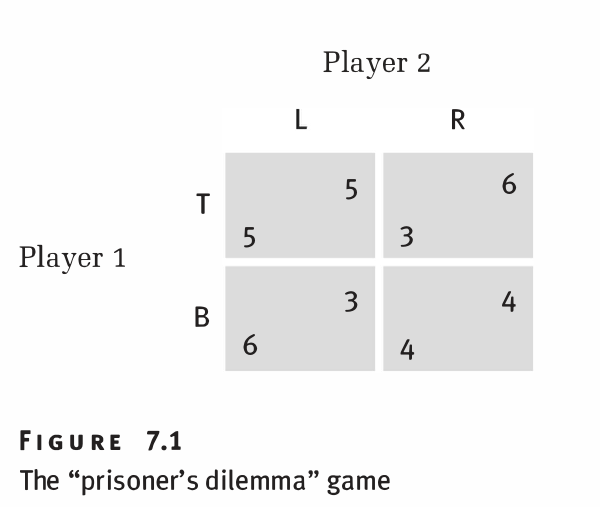
\includegraphics[width=0.42\linewidth]{figures/cabral-7-1.png}
\end{center}
\end{referencia}
\resolespaco

% ---------------------------------------------------------------------------
\exercicio[2]{Grim Trigger}{Foundations}{Tadelis (2013), \emph{Game Theory: An Introduction}, Ch.~10
``Repeated Games'', Exercise 10.2 ``Grim Trigger'', p.~215 [PDF 234]. No answer in the book.
Reproduced verbatim.}

\rot{10.2}\textbf{Grim Trigger:} Consider the infinitely repeated game with discount factor
$\delta < 1$ of the following variant of the Prisoner's Dilemma:
\jogo{Player 1}{Player 2}{\begin{tabular}{c|c|c|c|}
\hd{} & \hd{$L$} & \hd{$C$} & \hd{$R$}\\\cline{2-4}
$T$ & 6, 6 & $-1$, 7 & $-2$, 8\\\cline{2-4}
$M$ & 7, $-1$ & 4, 4 & $-1$, 5\\\cline{2-4}
$B$ & 8, $-2$ & 5, $-1$ & 0, 0\\\cline{2-4}
\end{tabular}}
\begin{partes}
\item For which values of the discount factor $\delta$ can the players support the pair of actions
$(M, C)$ played in every period?
\item For which values of the discount factor $\delta$ can the players support the pair of actions
$(T, L)$ played in every period? Why is your answer different from that for (a)?
\end{partes}
\resolespaco

% ---------------------------------------------------------------------------
\exercicio[2]{Infinitely Repeated Prisoner's Dilemma Game}{Foundations}{Muñoz-Garcia \& Toro-Gonzalez
(2019), \emph{Strategy and Game Theory: Practice Exercises with Answers}, 2nd ed., Ch.~6 ``Repeated
Games and Correlated Equilibria'', Exercise 1 ``Infinitely Repeated Prisoner's Dilemma
Game''$^{\mathrm{A}}$, p.~274 [PDF 285]. Worked answer in the book, right after the statement.
Reproduced verbatim (statement only); Table 6.1 rebuilt from the same page.}

Consider the infinitely repeated version of the following prisoner's dilemma game, where C denotes
confess and NC represents not confess (Table 6.1):

\textbf{Part (a)} Can players support the cooperative outcome (NC, NC) as a SPNE by using
tit-for-tat strategies, whereby players punish deviations from NC in a past period by reverting to
the stage-game Nash equilibrium where they both confess (C, C) for just one period, and then
returning to cooperation?

\textbf{Part (b)} Consider now that players play tit-for-tat, but reverting to the stage-game Nash
equilibrium where they both confess (C, C) for two periods, and then players return to cooperation.
Can the cooperative outcome (NC, NC) be supported as a SPNE?

\textbf{Part (c)} Suppose that players use strategies that punish deviation from cooperation by
reverting to the stage-game Nash equilibrium for ten periods before returning to cooperation.
Compute the threshold discount factor, $\delta$, above which cooperation can be sustained as a SPNE
of the infinitely repeated game.
\jogo{Player 1}{Player 2}{\begin{tabular}{c|c|c|}
\hd{} & \hd{C} & \hd{NC}\\\cline{2-3}
C & 2, 2 & 6, 0\\\cline{2-3}
NC & 0, 6 & 3, 3\\\cline{2-3}
\end{tabular}}
\vspace{-6pt}\begin{center}\small\textit{Table 6.1} Prisoner's dilemma game\end{center}
\resolespaco

% ---------------------------------------------------------------------------
\exercicio[3]{Representing Feasible, Individually Rational Payoffs}{Exam level}{Muñoz-Garcia \&
Toro-Gonzalez (2019), \emph{Strategy and Game Theory: Practice Exercises with Answers}, 2nd ed.,
Ch.~6 ``Repeated Games and Correlated Equilibria'', Exercise 9 ``Representing Feasible,
Individually Rational Payoffs''$^{\mathrm{C}}$, p.~305 [PDF 316]. Worked answer in the book, right
after the statement. Reproduced verbatim (statement only); Table 6.6, printed inside the answer on
the same page, rebuilt.}

Consider an infinitely-repeated game where the stage game is depicted Table 6.6. Player 1 chooses
rows and player 2 chooses columns. Players discount the future using a common discount factor
$\delta$.

\textbf{Part (a)} What outcomes in the stage-game are consistent with Nash equilibrium play?

\textbf{Part (b)} Let $v_1$ and $v_2$ be the repeated game payoffs to player 1 and player 2
respectively. Draw the set of feasible payoffs from the repeated game, explaining any normalization
you use.

\textbf{Part (c)} Find the set of individually rational feasible set of payoffs.

\textbf{Part (d)} Find a Nash equilibrium in which the players obtain (9, 9) each period. What
restrictions on $\delta$ are necessary?
\jogo{Player 1}{Player 2}{\begin{tabular}{c|c|c|}
\hd{} & \hd{$L$} & \hd{$R$}\\\cline{2-3}
$U$ & 9, 9 & 1, 10\\\cline{2-3}
$D$ & 10, 1 & 7, 7\\\cline{2-3}
\end{tabular}}
\vspace{-6pt}\begin{center}\small\textit{Table 6.6} Simultaneous-move game\end{center}
\resolespaco

% ---------------------------------------------------------------------------
\exercicio[3]{Not-So-Grim Trigger}{Exam level}{Tadelis (2013), \emph{Game Theory: An Introduction},
Ch.~10 ``Repeated Games'', Exercise 10.3 ``Not-So-Grim Trigger'', pp.~215--216 [PDF 234--235]. No
answer in the book. Reproduced verbatim, with the book's footnote 12 (p.~216). Here $T$ is the
length of the punishment.}

\rot{10.3}\textbf{Not-So-Grim Trigger:} Consider the infinitely repeated Prisoner's Dilemma with
discount factor $\delta < 1$ described by the following matrix:
\jogo{Player 1}{Player 2}{\begin{tabular}{c|c|c|}
\hd{} & \hd{$m$} & \hd{$f$}\\\cline{2-3}
$M$ & 4, 4 & $-1$, 5\\\cline{2-3}
$F$ & 5, $-1$ & 1, 1\\\cline{2-3}
\end{tabular}}
Instead of using grim-trigger strategies to support a pair of actions $(a_1, a_2)$ other than
$(F, f)$ as a subgame-perfect equilibrium, assume that the players wish to choose a less draconian
punishment called a ``length-$T$ punishment'' strategy. If there is a deviation from $(a_1, a_2)$
then the players will play $(F, f)$ for $T$ periods and then resume playing $(a_1, a_2)$. Let
$\delta_T$ be the critical discount factor so that if $\delta > \delta_T$ then the adequately
defined strategies will implement the desired path of play with length-$T$ punishment as the
threat.
\begin{partes}
\item Let $T = 1$. What is the critical value $\delta_1$ to support the pair of actions $(M, m)$
played in every period?
\item Let $T = 2$. What is the critical value $\delta_T$ to support the pair of actions $(M, m)$
played in every period?$^{12}$
\item Compare the two critical values in (a) and (b). How do they differ and what is the intuition
for this?
\end{partes}
{\small $^{12}$\,Hint: You should encounter an equation of the form $a\delta^3 - (a + 1)\delta + 1 = 0$,
for which it is easy to see that $\delta = 1$ is a root. In this case you know that the equation can
be written in the form $(\delta - 1)(a\delta^2 + a\delta - 1) = 0$, and you can solve for the other
relevant root of the cubic equation.\par}
\resolespaco

% ---------------------------------------------------------------------------
\exercicio[4]{Multistage Practice}{Exam level}{Tadelis (2013), \emph{Game Theory: An Introduction},
Ch.~9 ``Multistage Games'', Exercise 9.1 ``Multistage Practice'', pp.~186--187 [PDF 205--206]. No
answer in the book. Reproduced verbatim.}

\rot{9.1}\textbf{Multistage Practice:} Consider the following simultaneous-move game that is played
twice (the players observe the first-period outcome prior to the second-period play):
\jogo{Player 1}{Player 2}{\begin{tabular}{c|c|c|c|}
\hd{} & \hd{$L$} & \hd{$C$} & \hd{$R$}\\\cline{2-4}
$T$ & 10, 10 & 2, 12 & 0, 13\\\cline{2-4}
$M$ & 12, 2 & 5, 5 & 0, 0\\\cline{2-4}
$B$ & 13, 0 & 0, 0 & 1, 1\\\cline{2-4}
\end{tabular}}
\begin{partes}
\item Find all the pure-strategy subgame-perfect equilibria with no discounting ($\delta = 1$). Be
precise in defining history-contingent strategies for both players.
\item For each of the equilibria you found in (a), find the smallest discount factor that supports
it.
\end{partes}
\resolespaco

% ---------------------------------------------------------------------------
\exercicio[4]{Reaching a non-Nash payoff in the first stage}{Exam level}{Gibbons (1992), \emph{Game
Theory for Applied Economists}, Ch.~2 ``Dynamic Games of Complete Information'', \S2.6 Problems
(Section 2.3), Problem 2.11, p.~135 [PDF 142]. No answer in the book (Muñoz-Garcia \&
Toro-Gonzalez Ch.~6 Ex.~7, p.~299, works the same game). Reproduced verbatim.}

\rot{2.11.}The simultaneous-move game (below) is played twice, with the outcome of the first stage
observed before the second stage begins. There is no discounting. Can the payoff $(4, 4)$ be achieved
in the first stage in a pure-strategy subgame-perfect Nash equilibrium? If so, give strategies that
do so. If not, prove why not.
\begin{center}\begin{tabular}{c|c|c|c|}
\hd{} & \hd{$L$} & \hd{$C$} & \hd{$R$}\\\cline{2-4}
$T$ & 3, 1 & 0, 0 & 5, 0\\\cline{2-4}
$M$ & 2, 1 & 1, 2 & 3, 1\\\cline{2-4}
$B$ & 1, 2 & 0, 1 & 4, 4\\\cline{2-4}
\end{tabular}\end{center}
\resolespaco

% ---------------------------------------------------------------------------
\exercicio[4]{Asymmetric Patience 1}{Exam level}{Tadelis (2013), \emph{Game Theory: An Introduction},
Ch.~11 ``Strategic Bargaining'', Exercise 11.5 ``Asymmetric Patience 1'', pp.~236--237 [PDF
255--256]. No answer in the book. Reproduced verbatim.}

\rot{11.5}\textbf{Asymmetric Patience 1:} Consider a three-period sequential (alternating-offer)
bargaining model in which two players have to split a pie worth 1 (starting with player 1 making
the offer). Now the players have different discount factors, $\delta_1$ and $\delta_2$.
\begin{partes}
\item Compute the outcome of the unique subgame-perfect equilibrium.
\item Show that when $\delta_1 = \delta_2$ player 1 has an advantage.
\item What conditions on $\delta_1$ and $\delta_2$ give player 2 an advantage? Why?
\end{partes}

\begin{referencia}{the alternating-offer bargaining model this exercise modifies (``Now the
players have different discount factors''): Tadelis (2013), Ch.~11 ``Strategic Bargaining'',
p.~221 [PDF 240]. Reproduced verbatim (excerpts); with $\delta_1 \neq \delta_2$, player $i$
discounts with $\delta_i$.}
In the first round:
\begin{itemize}[leftmargin=1.6em]
\item Player 1 offers shares $(x, 1 - x)$, where player 1 receives $x$ and player 2 receives $1 - x$.
\item Player 2 then chooses to accept, causing the game to end with payoffs $v_1 = x$ and
$v_2 = 1 - x$, or reject, causing the game to move to the second round.
\end{itemize}
In the second round:
\begin{itemize}[leftmargin=1.6em]
\item A share $1 - \delta$ of the pie is dissipated (the pie is discounted with discount factor
$0 < \delta < 1$).
\item Player 2 offers shares $(x, 1 - x)$, where player 1 receives $x$ and player 2 receives $1 - x$.
\item Player 1 chooses to accept, causing the game to end with payoffs $v_1 = \delta x$ and
$v_2 = \delta(1 - x)$, or reject, causing the game to move to the third round.
\end{itemize}
In the third round and beyond:
\begin{itemize}[leftmargin=1.6em]
\item The game continues in the same way, where following rejection in an odd period player 2 gets
to offer in the next even period, and vice versa.
\item Each period has further discounting of the pie, so that in period $t$ the total pie is worth
$\delta^{t-1}$.
\end{itemize}
[\ldots] Assume for now that the game ends in some prespecified final period $T$, which will be
reached if the players did not reach an agreement in the $T - 1$ periods that preceded $T$.
Furthermore assume that period $T$ is a ``hard deadline,'' so that both players receive a payoff of
zero if they fail to reach an agreement in this last period.
\end{referencia}
\resolespaco

% ---------------------------------------------------------------------------
\exercicio[4]{Diluted Happiness}{Advanced}{Tadelis (2013), \emph{Game Theory: An Introduction}, Ch.~10
``Repeated Games'', Exercise 10.7 ``Diluted Happiness'', pp.~217--218 [PDF 236--237]. No answer in
the book. Reproduced verbatim.}

\rot{10.7}\textbf{Diluted Happiness:} Consider a relationship between a bartender and a customer. The
bartender serves bourbon to the customer and chooses $x \in [0, 1]$, which is the proportion of
bourbon in the drink served, while $1 - x$ is the proportion of water. The cost of supplying such a
drink (standard 4-ounce glass) is $cx$, where $c > 0$. The customer, without knowing $x$, decides on
whether or not to buy the drink at the market price $p$. If he buys the drink his payoff is
$vx - p$, and the bartender's payoff is $p - cx$. Assume that $v > c$ and all payoffs are common
knowledge. If the customer does not buy the drink he gets 0 and the bartender gets $-cx$. Because
the customer has some experience, once the drink is bought and he tastes it, he learns the value of
$x$, but this is only after he pays for the drink.
\begin{partes}
\item Find all the Nash equilibria of this game.
\item Now assume that the customer is visiting town for 10 days, and this ``bar game'' will be
played on each of the 10 evenings that the customer is in town. Assume that each player tries to
maximize the (nondiscounted) sum of his stage payoffs. Find all the subgame-perfect equilibria of
this game.
\item Now assume that the customer is a local, and the players perceive the game as repeated
infinitely many times. Assume that each player tries to maximize the discounted sum of his stage
payoffs, where the discount rate is $\delta \in (0, 1)$. What is the range of prices $p$ (expressed
in the parameters of the problem) for which there exists a subgame-perfect equilibrium in which
every day the bartender chooses $x = 1$ and the customer buys at the price $p$?
\item For which values of $\delta$ (expressed in the parameters of the problem) can the price range
that you found in (c) exist?
\end{partes}
\resolespaco

% ---------------------------------------------------------------------------
\needspace{20\baselineskip}
\exercicio[5]{Rubinstein's strategies are subgame-perfect}{Advanced}{Gibbons (1992), \emph{Game Theory
for Applied Economists}, Ch.~2 ``Dynamic Games of Complete Information'', \S2.6 Problems (Section
2.4), Problem 2.20, pp.~137--138 [PDF 144--145]. No answer in the book. Reproduced verbatim.}

\rot{2.20.}Consider the following strategies in the infinite-horizon version of Rubinstein's
bargaining model. (Recall the notational convention that the offer $(s, 1 - s)$ means that Player 1
will get $s$ and Player 2 will get $1 - s$, independent of who made the offer.) Let
$s^* = 1/(1 + \delta)$. Player 1 always offers $(s^*, 1 - s^*)$ and accepts an offer $(s, 1 - s)$
only if $s \ge \delta s^*$. Player 2 always offers $(1 - s^*, s^*)$ and accepts an offer
$(s, 1 - s)$ only if $1 - s \ge \delta s^*$. Show that these strategies are a Nash equilibrium.
Show that this equilibrium is subgame-perfect.

\begin{referencia}{``the infinite-horizon version of Rubinstein's bargaining model'': Gibbons (1992),
\S2.1.D ``Sequential Bargaining'', pp.~68--70 [PDF 75--77]. Reproduced verbatim (excerpts); footnote~7
(on the discount factor as $\delta = 1/(1+r)$) omitted.}
Players 1 and 2 are bargaining over one dollar. They alternate in making offers: first player 1
makes a proposal that player 2 can accept or reject; if 2 rejects then 2 makes a proposal that 1 can
accept or reject; and so on. Once an offer has been rejected, it ceases to be binding and is
irrelevant to the subsequent play of the game. Each offer takes one period, and the players are
impatient: they discount payoffs received in later periods by the factor $\delta$ per period, where
$0 < \delta < 1$.

A more detailed description of the timing of the three-period bargaining game is as follows.
\begin{itemize}[leftmargin=2.6em]
\item[(1a)] At the beginning of the first period, player 1 proposes to take a share $s_1$ of the
dollar, leaving $1 - s_1$ for player 2.
\item[(1b)] Player 2 either accepts the offer (in which case the game ends and the payoffs $s_1$ to
player 1 and $1 - s_1$ to player 2 are immediately received) or rejects the offer (in which case
play continues to the second period).
\item[(2a)] At the beginning of the second period, player 2 proposes that player 1 take a share
$s_2$ of the dollar, leaving $1 - s_2$ for player 2. (Note the convention that $s_t$ always goes to
player 1, regardless of who made the offer.)
\item[(2b)] Player 1 either accepts the offer (in which case the game ends and the payoffs $s_2$ to
player 1 and $1 - s_2$ to player 2 are immediately received) or rejects the offer (in which case
play continues to the third period).
\item[(3)] At the beginning of the third period, player 1 receives a share $s$ of the dollar,
leaving $1 - s$ for player 2, where $0 < s < 1$.
\end{itemize}
[\ldots] Now consider the infinite-horizon case. The timing is as described previously, except that
the exogenous settlement in step (3) is replaced by an infinite sequence of steps (3a), (3b), (4a),
(4b), and so on. Player 1 makes the offer in odd-numbered periods, player 2 in even-numbered;
bargaining continues until one player accepts an offer.
\end{referencia}
\resolespaco
